\documentclass[12pt,a4paper]{report}
\usepackage{graphicx}
\usepackage{amsmath}
\usepackage{fancyhdr}
\usepackage{cite}
\usepackage{framed}
\usepackage{a4wide}
\usepackage{float}
\usepackage{epsfig}
\usepackage{longtable}
\usepackage{enumerate}
\usepackage{afterpage}
\usepackage{multirow}
\usepackage{ragged2e}
\usepackage{gensymb}
\usepackage{amsfonts} 
\usepackage[left=3.5cm,top=1.5cm,right=3cm,bottom=4cm]{geometry}
\usepackage{setspace}           
\usepackage{float}
\usepackage{txfonts}
\usepackage{lipsum}

\newcommand{\Usefont}[1]{\fontfamily{#1}\selectfont}

\usepackage{lscape} % for landscape tables
\renewcommand{\baselinestretch}{1.7} 

\usepackage{blindtext}
\usepackage{xpatch}
\usepackage{url}
\usepackage{leqno}
\usepackage{subcaption}
\usepackage{listings} % for listing code in the report
%\usepackage{mips}
\usepackage{color}

\definecolor{codegreen}{rgb}{0,0.6,0}
\definecolor{gray}{rgb}{0.5,0.5,0.5}
\definecolor{mauve}{rgb}{0.58,0,0.82}

\lstset{ %
	basicstyle=\footnotesize,       % the size of the fonts that are used for the code
	numbers=left,                   % where to put the line-numbers
	numberstyle=\tiny\color{gray},  % the style that is used for the line-numbers
	stepnumber=1,                   % the step between two line-numbers. If it's 1, each line
	% will be numbered
	numbersep=5pt,                  % how far the line-numbers are from the code
	backgroundcolor=\color{white},  % choose the background color. You must add \usepackage{color}
	showspaces=false,               % show spaces adding particular underscores
	showstringspaces=false,         % underline spaces within strings
	showtabs=false,                 % show tabs within strings adding particular underscores
	%frame=single,                   % adds a frame around the code
	rulecolor=\color{black},        % if not set, the frame-color may be changed on line-breaks within not-black text (e.g. commens (green here))
	tabsize=4,                      % sets default tabsize to 2 spaces
	captionpos=b,                   % sets the caption-position to bottom
	breaklines=true,                % sets automatic line breaking
	breakatwhitespace=false,        % sets if automatic breaks should only happen at whitespace
	%title=\lstname,                 % show the filename of files included with \lstinputlisting;
	% also try caption instead of title
	keywordstyle=\color{blue},          % keyword style
	commentstyle=\color{codegreen},       % comment style
	stringstyle=\color{mauve},         % string literal style
	escapeinside={\%*}{*)},            % if you want to add a comment within your code
	morekeywords={*,...}               % if you want to add more keywords to the set
}


\linespread{1.5}
\usepackage[intoc, english]{nomencl}
\hyphenpenalty=5000
\tolerance=1000
\usepackage[nottoc]{tocbibind}
\bibliographystyle{IEEEtran}
\renewcommand{\bibname}{References}

%*******************************************************************
%                        Header and Footer   
% This is not required in Technical reports submitted to CET ECE department.
% Please leave it commented                       
%*******************************************************************
%\pagestyle{fancy}
%\fancyhead{}
%\header and footer section
%\renewcommand\headrulewidth{0.1pt}
%\fancyhead[L]{\footnotesize \leftmark}
%\fancyhead[R]{\footnotesize \thepage}
%\renewcommand\headrulewidth{0pt}
%\fancyfoot[R]{\small College of Engineering Trivandrum}
%\renewcommand\footrulewidth{0.1pt}
%\fancyfoot[C]{2020 - 2021}
%\fancyfoot[L]{\small Title of the Seminar/Project}
%*******************************************************************


%*********************Figures*****************************
% Save all figures in the folder figures and include them in your 
% report using the command \includegraphics{figure-name}

\graphicspath{{figures/}}

% figure files can be in jpeg,jpg, png or pdf formats
%*******************************************************************


\begin{document}
		
%****The entries in this section are to be filled in by the student with appropriate values *************

% These values are used thoroughout the report 
% please fill in the appropriate values in the brackets {}

\gdef \title{DROWSY DRIVER DETECTION USING 8051} % Project title
\gdef \student{Vinayak Prakash}	 %student name
\gdef \studentroll{LTVE22EC074} % Project batch member 1 ktu id
\gdef \dept{Electronics and Communication Engineering} %Department
\gdef \degree{Bachelor of Technology} %degree
\gdef \branch{Electronics and Communication Engineering} %branch
\gdef \college{College of Engineering Trivandrum} % Name of the College
\gdef \collegeplace{Trivandrum} % Location of the College

\gdef \facultyA{Prof. Joaquim Ignatious Monteiro} %Project guide
\gdef \facultyAdes{Assistant Professor}%project guide designation

\gdef \acadyear{2023 - 24} % Academic year
\gdef \month{May 2024} %Month of Report submission
\gdef \date{15-02-2024} %Date of signing the declaration

%*******************************************************************
% The font pages. The source tex files are there in the folder
%==================================coverpage.tex================================


\newenvironment{coverpage}
\thispagestyle{empty}
\begin{titlepage}
	\begin{center}
		{\Usefont{phv} \Large \bf \title \par}
		\vspace*{40pt}
		\large \em \Usefont{pzc}{ 
			A Course Project Report \par
			Submitted to the APJ Abdul Kalam Technological University\\
			in partial fulfillment of requirements for the award of degree}\\ [.15\baselineskip] \par
		\Usefont{ppl} {\bfseries  \degree}\\
		in\\
		{\Usefont{ppl} {\bfseries \branch}}\\
		by\\
		\bf {\student}\\(\studentroll)\\
		
		\vspace*{40pt}
		\centering
		\begin{figure}[h!]
			\centerline{
\includegraphics[scale=0.6]{cet_logo}}
		\end{figure}
		
		\vspace*{\stretch{0.5}}
		\centering
		\bf {Computer Architecture and Microcontrollers}\\
		\bf {ECT 206}
		
		
		\vspace{\stretch{0.5}}
		\footnotesize{\bf DEPARTMENT OF ELECTRONICS AND COMMUNICATION ENGINEERING} \par
		\bf{COLLEGE OF ENGINEERING TRIVANDRUM} \par
		\bf{KERALA} \par
		\bf{\month}
	\end{center}		
\end{titlepage}	
 %Unless essential Do not edit this tex file



%%********************Certificate*******************

% To print name of only the project coordinator 1 in the certificate page
%==================================certificate1.tex================================
% To print name of only the seminar coordinator 1 in the certificate page

\newenvironment{certificate1}

	\newpage
	\begin{center}	
		%\vspace{1.5cm}
		
		\textbf{DEPT. OF ELECTRONICS \& COMMUNICATION ENGINEERING}	
		\textbf{COLLEGE OF ENGINEERING}	
		\textbf{TRIVANDRUM}
		
		\textbf{\acadyear} 
	\end{center}
	
	\begin{center}
		
\includegraphics[scale=0.5]{cet_logo}	
	\end{center}
	\begin{center}
		\textbf{CERTIFICATE}
	\end{center}
	
	This is to certify that the report entitled \textbf{\title} submitted by \textbf{\student}\hspace*{2pt}(\studentroll) to the APJ Abdul Kalam Technological University in partial fulfillment of the B.Tech.\ degree in \branch \hspace*{2pt} is a bonafide record of the course project work carried out by him under our guidance and supervision. This report in any form has not been submitted to any other University or Institute for any purpose.
	
	
	\begin{singlespace}
		
		\vspace*{1.3cm}
		
		\begin{flushright}
			%\centering{
			%\hline
			\textbf{\facultyA} \\ 
			\facultyAdes\\ 
			Dept.of ECE\\ 
			College of Engineering\\
			Trivandrum\\
		\end{flushright}
	\end{singlespace}
	
	\thispagestyle{empty}



 

% To print names of both the project coordinators in the certificate page
%%==================================certificate2.tex================================
% To print names of both the seminar coordinators in the certificate page
\newenvironment{certificate2}

\newpage
\begin{center}	
	%\vspace{1.5cm}
	
	\textbf{DEPT. OF ELECTRONICS \& COMMUNICATION ENGINEERING}	
	\textbf{COLLEGE OF ENGINEERING}	
	\textbf{TRIVANDRUM}
	
	\textbf{\acadyear} 
\end{center}

\begin{center}
	
\includegraphics[scale=0.5]{cet_logo}	
\end{center}
\begin{center}
	\textbf{CERTIFICATE}
\end{center}

This is to certify that the report entitled \textbf{\title} submitted by \textbf{\author} \hspace*{2pt}(\rollno), to the APJ Abdul Kalam Technological University in partial fulfillment of the B.Tech.\ degree in \branch \hspace*{2pt} is a bonafide record of the seminar work carried out by him under our guidance and supervision. This report in any form has not been submitted to any other University or Institute for any purpose.


\begin{singlespace}
	\vspace*{2cm}
	\begin{table}[h!]
		\centering
		\begin{tabular}{p{7cm} p{0.9cm} p{7cm}} 
			\textbf{\guide} && \textbf{\semcordinatorA} \\
			(Seminar Guide) &&  (Seminar Coordinator)\\
			\guidedes & & \semcordinatorAdes\\ 
			\deptabbr && \deptabbr\\ 
			\college & &\college\\
			\collegeplace && \collegeplace\\
		\end{tabular}
		
	\end{table}
	
	\vspace*{1.3cm}
	
	\begin{center}
		\begin{tabular}{p{7cm} p{0.9cm} p{7cm}} 
			%\hline
			\textbf{\semcordinatorB} && \textbf{\hod} \\
			\semcordinatorBdes & & \hoddes\\ 
			\deptabbr && \deptabbr\\ 
			\college & &\college\\
			\collegeplace && \collegeplace\\
		\end{tabular}
	\end{center}
\end{singlespace}

\thispagestyle{empty}



 %Please uncomment this and comment the previous line

%%***************************************************


%%==================================declaration.tex================================
%
\newpage
\newenvironment{declaration}
\thispagestyle{empty}
\begin{center}
\vspace*{50pt}
\textbf{DECLARATION}\\
\end{center}
We hereby declare that the project report {\bf{\title}}, submitted for partial fulfillment of the requirements for the award of degree of Bachelor of Technology of the APJ Abdul Kalam Technological University, Kerala is a bonafide work done by us under supervision of \guide \hspace*{2pt} \par
This submission represents our ideas in our own words and where ideas or words of others have been included, we have adequately and accurately cited and referenced the original sources.\par 
We also declare that I have adhered to ethics of academic honesty and integrity and have not misrepresented or fabricated any data or idea or fact or source in my submission. We understand that any violation of the above will be a cause for disciplinary action by the institute and/or the
University and can also evoke penal action from the sources which have thus not been properly cited or from whom proper permission has not been obtained. This report has not been previously formed the basis for the award of any degree, diploma or similar title of any other University.

\noindent \begin{minipage}{0.45\linewidth}
\begin{flushleft}
\vspace{2.5cm}

\collegeplace \\
\date

\end{flushleft} 
\end{minipage}
\hfill
\begin{minipage}{0.45\linewidth}
\begin{flushright}                                      
\vspace{1.5cm}

\textbf{\studentA}\\
\textbf{\studentB}\\


\end{flushright} 
\end{minipage}
\thispagestyle{empty}
 %Unless essential Do not edit this tex file

\pagenumbering{roman} 

%%********************************Abstract***********************
%============================= abstract.tex================================
\chapter*{Abstract}%
%\addcontentsline{toc}{chapter}{\numberline{}Abstract}%
\addcontentsline{toc}{chapter}{Abstract}%

This document contains essential templates required to write technical
reports using \LaTeX. This template may be used for the preparation of B.Tech seminar reports of APJ Abdul Kalam Technological University, Kerala. Also minimum working examples to create equations, include figure, include table, table of contents symbols list and bibliographic citation in a \LaTeX\ document are provided.\\

Please note that this template is provided without warranty on an AS IS basis.\\
\begin{flushright}
	\textit{JIM}
\end{flushright}

\thispagestyle{plain}
%=======================================================================

 % Please type in the abstract in this tex file abstract.tex

%%***************************************************
% Default Acknowledgement page
%%==================================acknowledgement.tex=============================
\chapter*{Acknowledgement}%
\addcontentsline{toc}{chapter}{Acknowledgement}%

%\newenvironment{acknowledgement}


\par We take this opportunity to express my deepest sense of gratitude and sincere thanks to everyone who helped us to complete this work successfully. We express our sincere thanks to \hod, Head of Department, \dept, \college\hspace*{2pt} for providing  us with all the necessary facilities and support.\par

We would like to express my sincere gratitude to the \projcordinatorA, \hspace*{2pt} department of \hspace*{2pt} \dept, \hspace*{2pt} \college \hspace*{2pt} \collegeplace \hspace*{2pt} for the support and co-operation.

We would like to place on record my sincere gratitude to our project guide \facultyA,\hspace*{2pt}\facultyAdes,\hspace*{2pt}\dept,\hspace*{2pt}\college \hspace*{2pt} %and our external guide \guideext,\hspace*{2pt}\guideextdes, \hspace*{2pt} \guideextorg   
for the guidance and mentorship throughout this work.

Finally I thank my family, and friends who contributed to the succesful fulfilment of this seminar work.

\vspace*{30pt}
\begin{flushright}
	\textbf{\studentA}\\
	\textbf{\studentB}\\

\end{flushright}
\thispagestyle{plain}
  %Unless essential Do not edit this tex file


%%***************************************************
%%**If you have only one seminar coordinator faculty member
% please comment the above line and uncomment this line

%%==================================acknowledgement.tex=============================
\chapter*{Acknowledgement}%
\addcontentsline{toc}{chapter}{Acknowledgement}%

%\newenvironment{acknowledgement}


I take this opportunity to express my deepest sense of gratitude and sincere thanks to everyone who helped me to complete this work successfully. I express my sincere thanks to \textbf{ \hod}, Head of Department, \dept, \college\hspace*{2pt} \collegeplace \hspace*{2pt} for providing  me with all the necessary facilities and support.\par

 I would like to express my sincere gratitude to \textbf{\semcordinatorA}, \hspace*{2pt} department of \hspace*{2pt} \dept, \hspace*{2pt} \college \hspace*{2pt} \collegeplace \hspace*{2pt} for their support and co-operation.

\noindent I would like to place on record my sincere gratitude to my seminar guide \textbf{\guide},\hspace*{2pt}\guidedes,\hspace*{2pt}\dept,\hspace*{2pt}\college \hspace*{2pt} for the guidance and mentorship throughout the course.

Finally I thank my family, and friends who contributed to the succesful fulfilment of this seminar work.

\vspace*{30pt}
\begin{flushright}
	\textbf{\author}
\end{flushright}
\thispagestyle{plain}
  %Unless essential Do not edit this tex file
%*******************************************************************

\thispagestyle{empty}
\newpage
    
%%**********************Table of Contents***********************
\tableofcontents
\listoffigures
%\listoftables
%%==================================symbols.tex================================
% List of Symbols
\chapter*{List of Symbols}
\addcontentsline{toc}{chapter}{List of Symbols}%
%\makeatletter
%
%\makeatother
%%\newcommand{\abbrlabel}[1]{\makebox[3cm][l]{\textbf{#1}\ \tocfill}}

\newenvironment{symbols}

		
\begin{itemize}	\setlength{\itemsep}{0pt}
	\item [$\Omega$] \text{Unit of Resistance}
	\item[$\varepsilon^{'}$]  Real part of dielectric constant 
	\item[$\mbox{c}$]	Speed of light
	\item[$\lambda$]	Wavelength
	\item[$\delta$] Delta
\end{itemize}
		
%\begin{symbols}
%	\item \symbol{$\Omega$} \text{Unit of Resistance}
	
%	\item \symbol{[$\mu$]} 	\text{Magnetic permeability}
%	\item[$\mu_0$]	Magnetic permeability of free space
%	\item[$\varepsilon$] Relative complex dielectric constant
%	\item[$\varepsilon^{'}$]  Real part of dielectric constant 
%	\item[$\varepsilon^{''}$] Imaginary part of dielectric constant 
%	\item[$\varepsilon_{s}$] Snow surface dielectric constant
%	\item[$\mbox{c}$]	Speed of light
%	\item[$\lambda$]	Wavelength
%	\item[$\tau$] Pulse length of SAR signal
%	\item[$\beta$]  Bandwidth of the SAR signal
%	\item[$\theta$ ] 	Orientation angle 
%	\item[$\theta_{i}$] 	Incidence or local incidence angle
%	\item[$\theta_{r}$]  Local refractive angle 
%	\item[$\delta A$]	Azimuth resolution of the SAR data
%	\item[$L$]    SAR antenna length
%	\item[$\mathbf{E}(\mathbf{r},t)$] Electric field vector
%	\item[$\mathbf{E_{pq}^s}$]	Scattered field vector
%	\item[$\rho(\mathbf{r}, t)$] Volume density of free charges
%	\item[$\mathbf{g}_\mathbf{E}$] Stokes vector


 %List of Symbols (Optional) comment if not required.
% symbold may be added in the file symbol.tex

%%********************Body of the report**********
% Arabic numbering is used in the body of the report

\cleardoublepage
\setcounter{page}{1}
\pagenumbering{arabic}

%%********************Chapter 1**********
\chapter{Introduction}
 
\noindent Road safety is a primary concern with driver fatigue being a major contributing factor to accidents. Drowsy driving can impair reaction time, judgment, and awareness, significantly increasing the risk of collisions. This project aims to develop a microcontroller-based drowsy driver detection system using an infrared (IR) sensor to enhance driver safety.
\par The 8051 microcontroller is a widely used microcontroller in embedded systems
due to its simplicity, versatility, and ease of programming. By leveraging its
capabilities, we can easily interface it with IR sensor module.
\par  The major components in this project are AT89S51, a IR Sensor Module
 
 \section{Problem statement}
Drowsy driving is a critical safety concern, contributing to a substantial number of road accidents. When drivers become fatigued, their reaction times decrease, judgment becomes impaired, and awareness of surroundings diminishes. This significantly increases the risk of collisions and potentially fatal outcomes.

\par Current solutions for drowsy driver detection may involve complex camera systems, physiological monitoring, or lane departure warning systems. However, these solutions can be expensive, intrusive, or have limitations in effectiveness.

\par There is a need for a simpler, more cost-effective, and driver-focused solution to detect drowsiness at an early stage. This system should provide an immediate and clear warning to the driver without requiring complex user interaction or additional visual displays within the vehicle.
 \section{Project objectives}
This project aims to develop a microcontroller-based drowsy driver detection system using an infrared (IR) sensor to address the problem of driver fatigue and enhance road safety. The specific objectives are:
\begin{itemize}
	\item \textbf {Design a system that utilizes an IR sensor to detect closed eyes.} The system should be able to reliably differentiate between open and closed eyes based on the change in reflected IR light.
	\item \textbf {Implement an 8051 microcontroller to process sensor data and trigger alerts.} The microcontroller will analyze sensor readings and activate the alert mechanism if closed-eye detection persists for a predetermined period.
	\item \textbf {Develop an audible alert system using a buzzer.} The chosen alert method should be clear, immediate, and effective in grabbing the driver's attention when drowsiness is detected.
	\item \textbf {Maintain a cost-effective and user-friendly design.} The system should prioritize affordability and ease of use while achieving its core functionality.
	\item \textbf {Promote driver awareness of drowsiness.}The timely buzzer alert aims to jolt the driver back to alertness and encourage them to take appropriate actions like pulling over for a rest.
\end{itemize}
 
%%********************Chapter 2**********
\chapter{Project Design and Testing}
By achieving these objectives, the project aims to deliver a fully functional and
user-friendly drowsy driver detector\\
THIS SECTION INCLUDES: \textbf{SOFTWARE IMPLEMENTATION}\\
 *WRITING CODE IN 8051 IN KIELuVISION\\
 *DEBUGGING CODE ON ANY ERROR\\
 *SIMULATION\\
 HEX FILE GENERATION\\
 \textbf{HARDWARE IMPLEMENTATION}\\
 BURN HEXFILE TO 8051 MICROCONTROLLER(USING ARDUINO AS ISP)
 CONNECT ALL OTHER COMPONENTS TO MAKE THE CIRCUIT FOR WORKING OF PROJECT.

\section{CODING :KEILUVISION}
 i have made the code using embedded C program,C language is generally preferred
BECAUSE C language code is often more readable and easier to understand compared
to assembly language code. It uses higher-level constructs, such as functions, variables,
and structured control flow, which make the code more modular and maintainable.
I have used 8051 keiluvision for simulation.


\subsection{CODE EXECUTION:keiluvision5}
I entered the embedded c code in keil.The code was executed and errors were rectified.
Then simulation was done using keil.
\begin{figure}[h!]
	\centering
	\begin{subfigure}[b]{0.4\textwidth}
		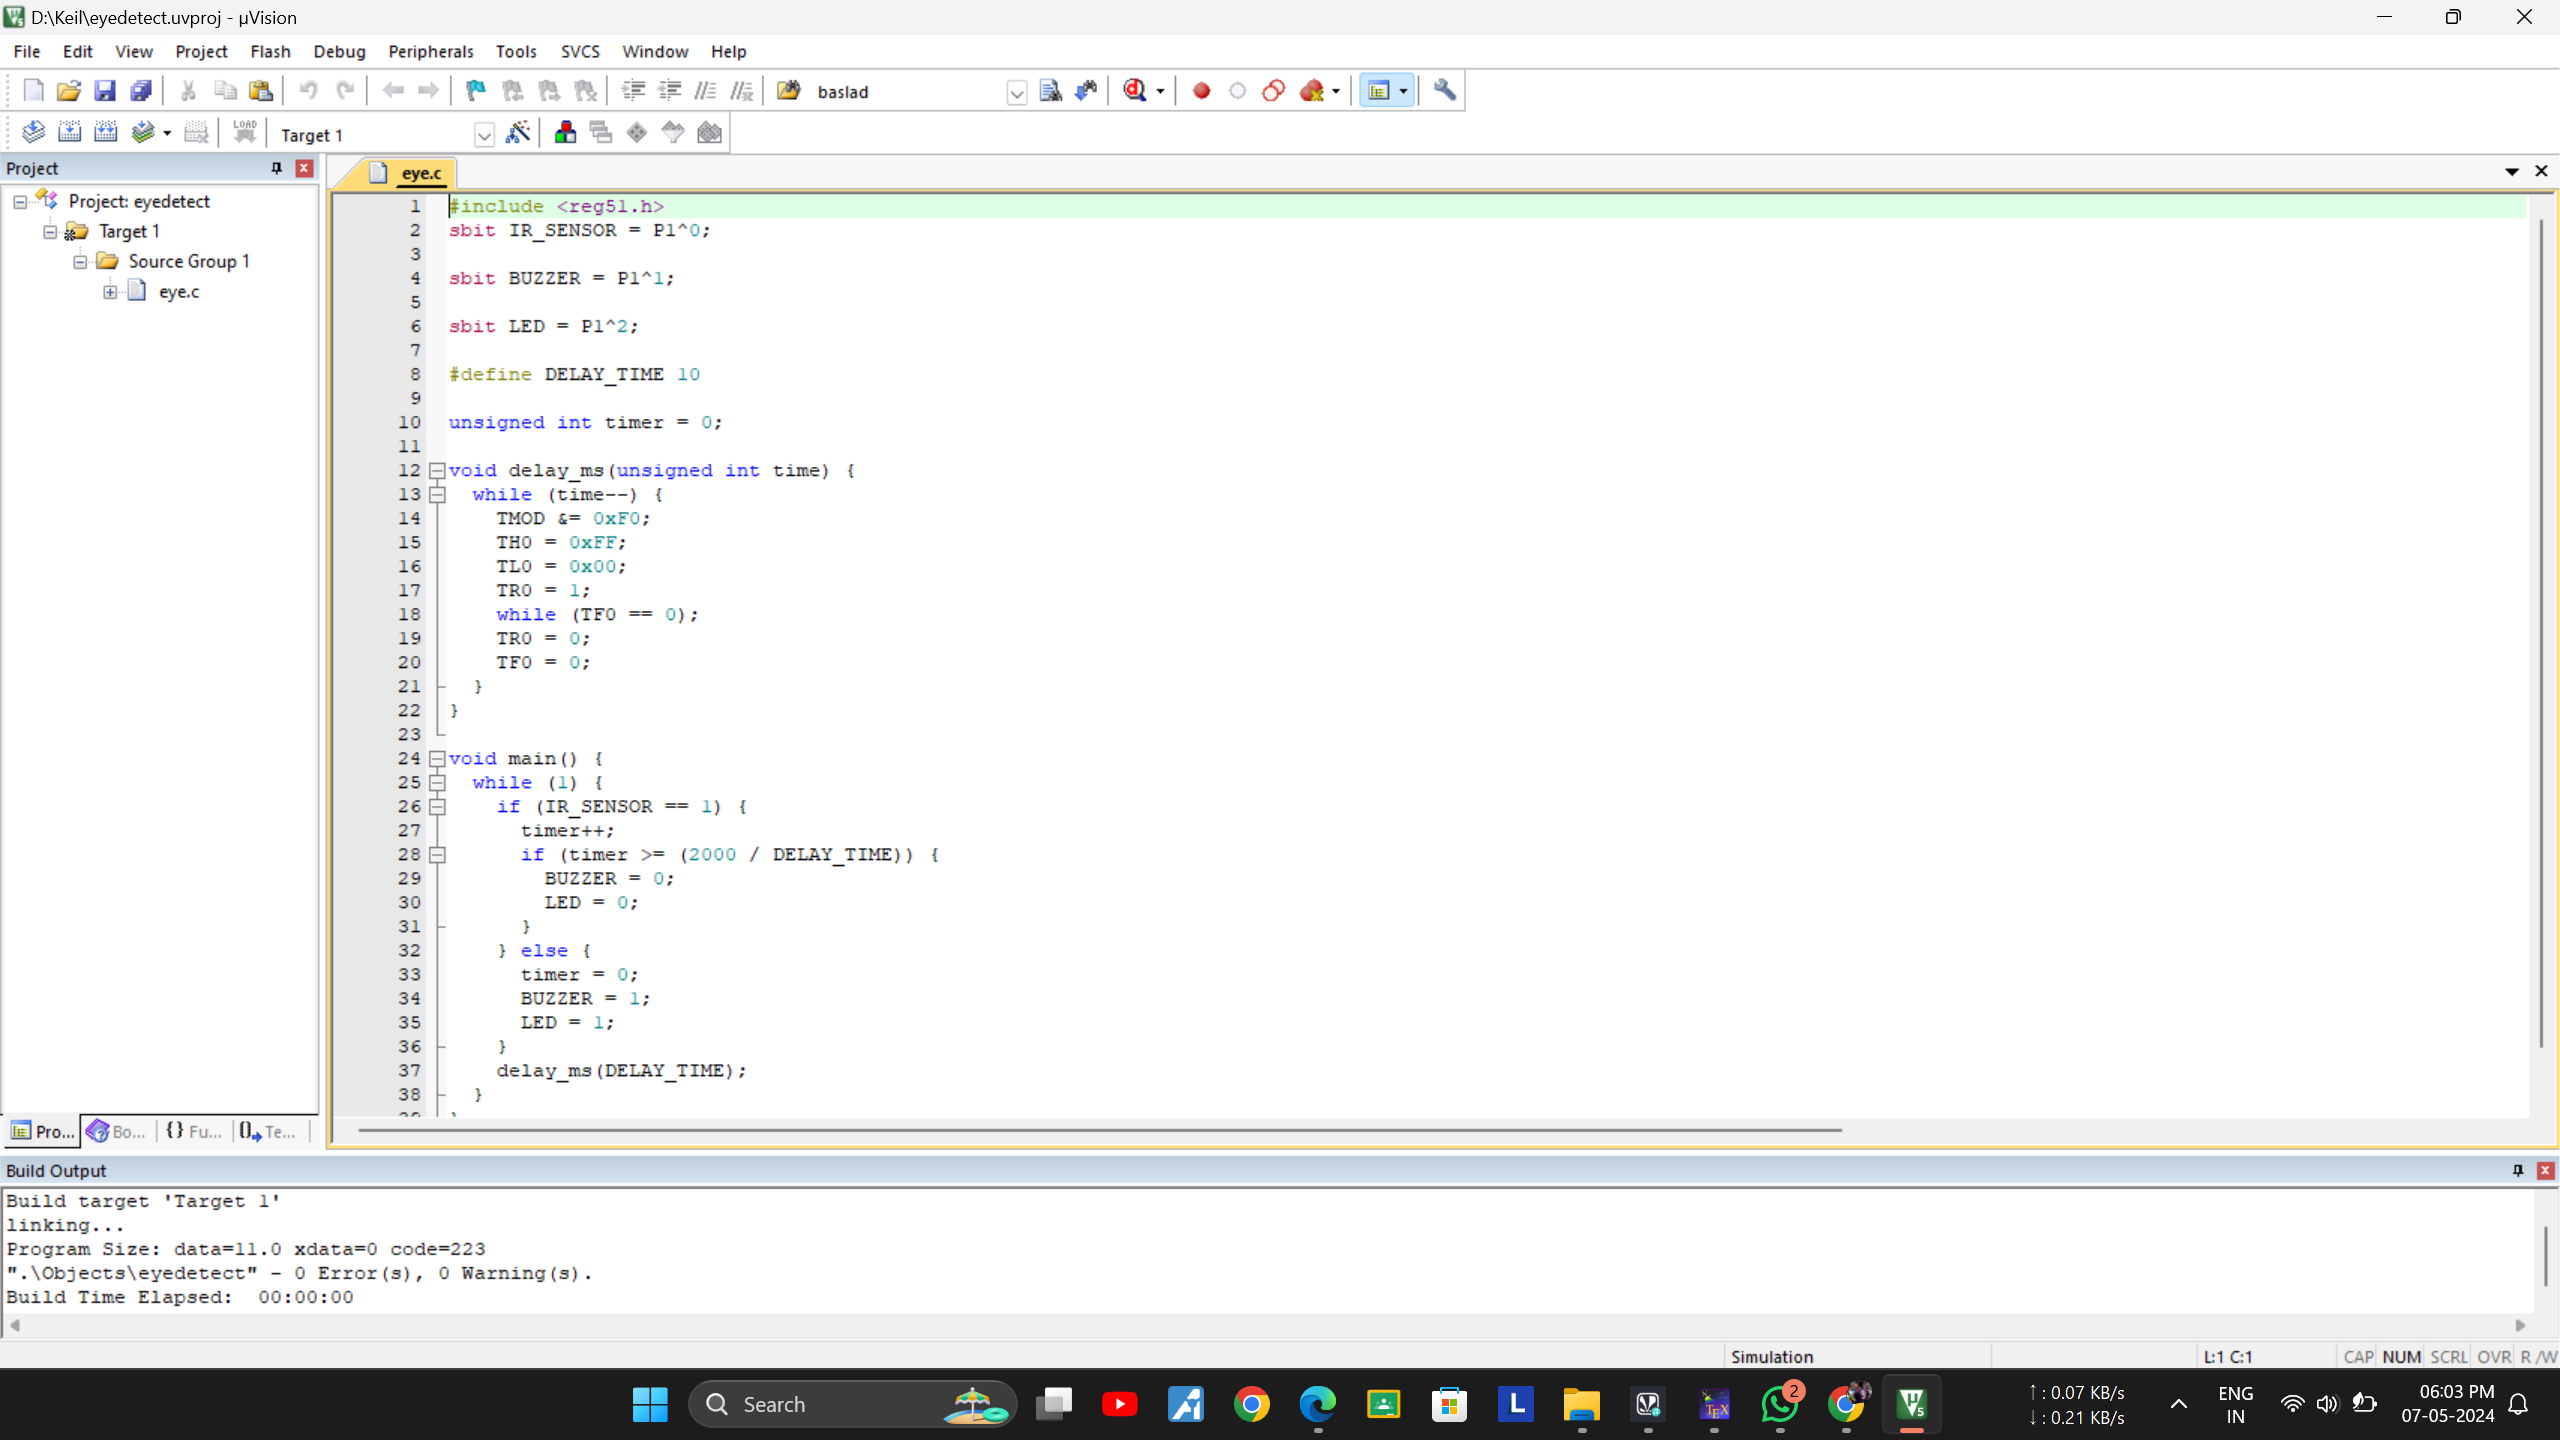
\includegraphics[width=\textwidth]{code_execution}
		\caption{code execution}
		\label{fig:1}
	\end{subfigure}
	\hspace{20mm}
	\begin{subfigure}[b]{0.4\textwidth}
		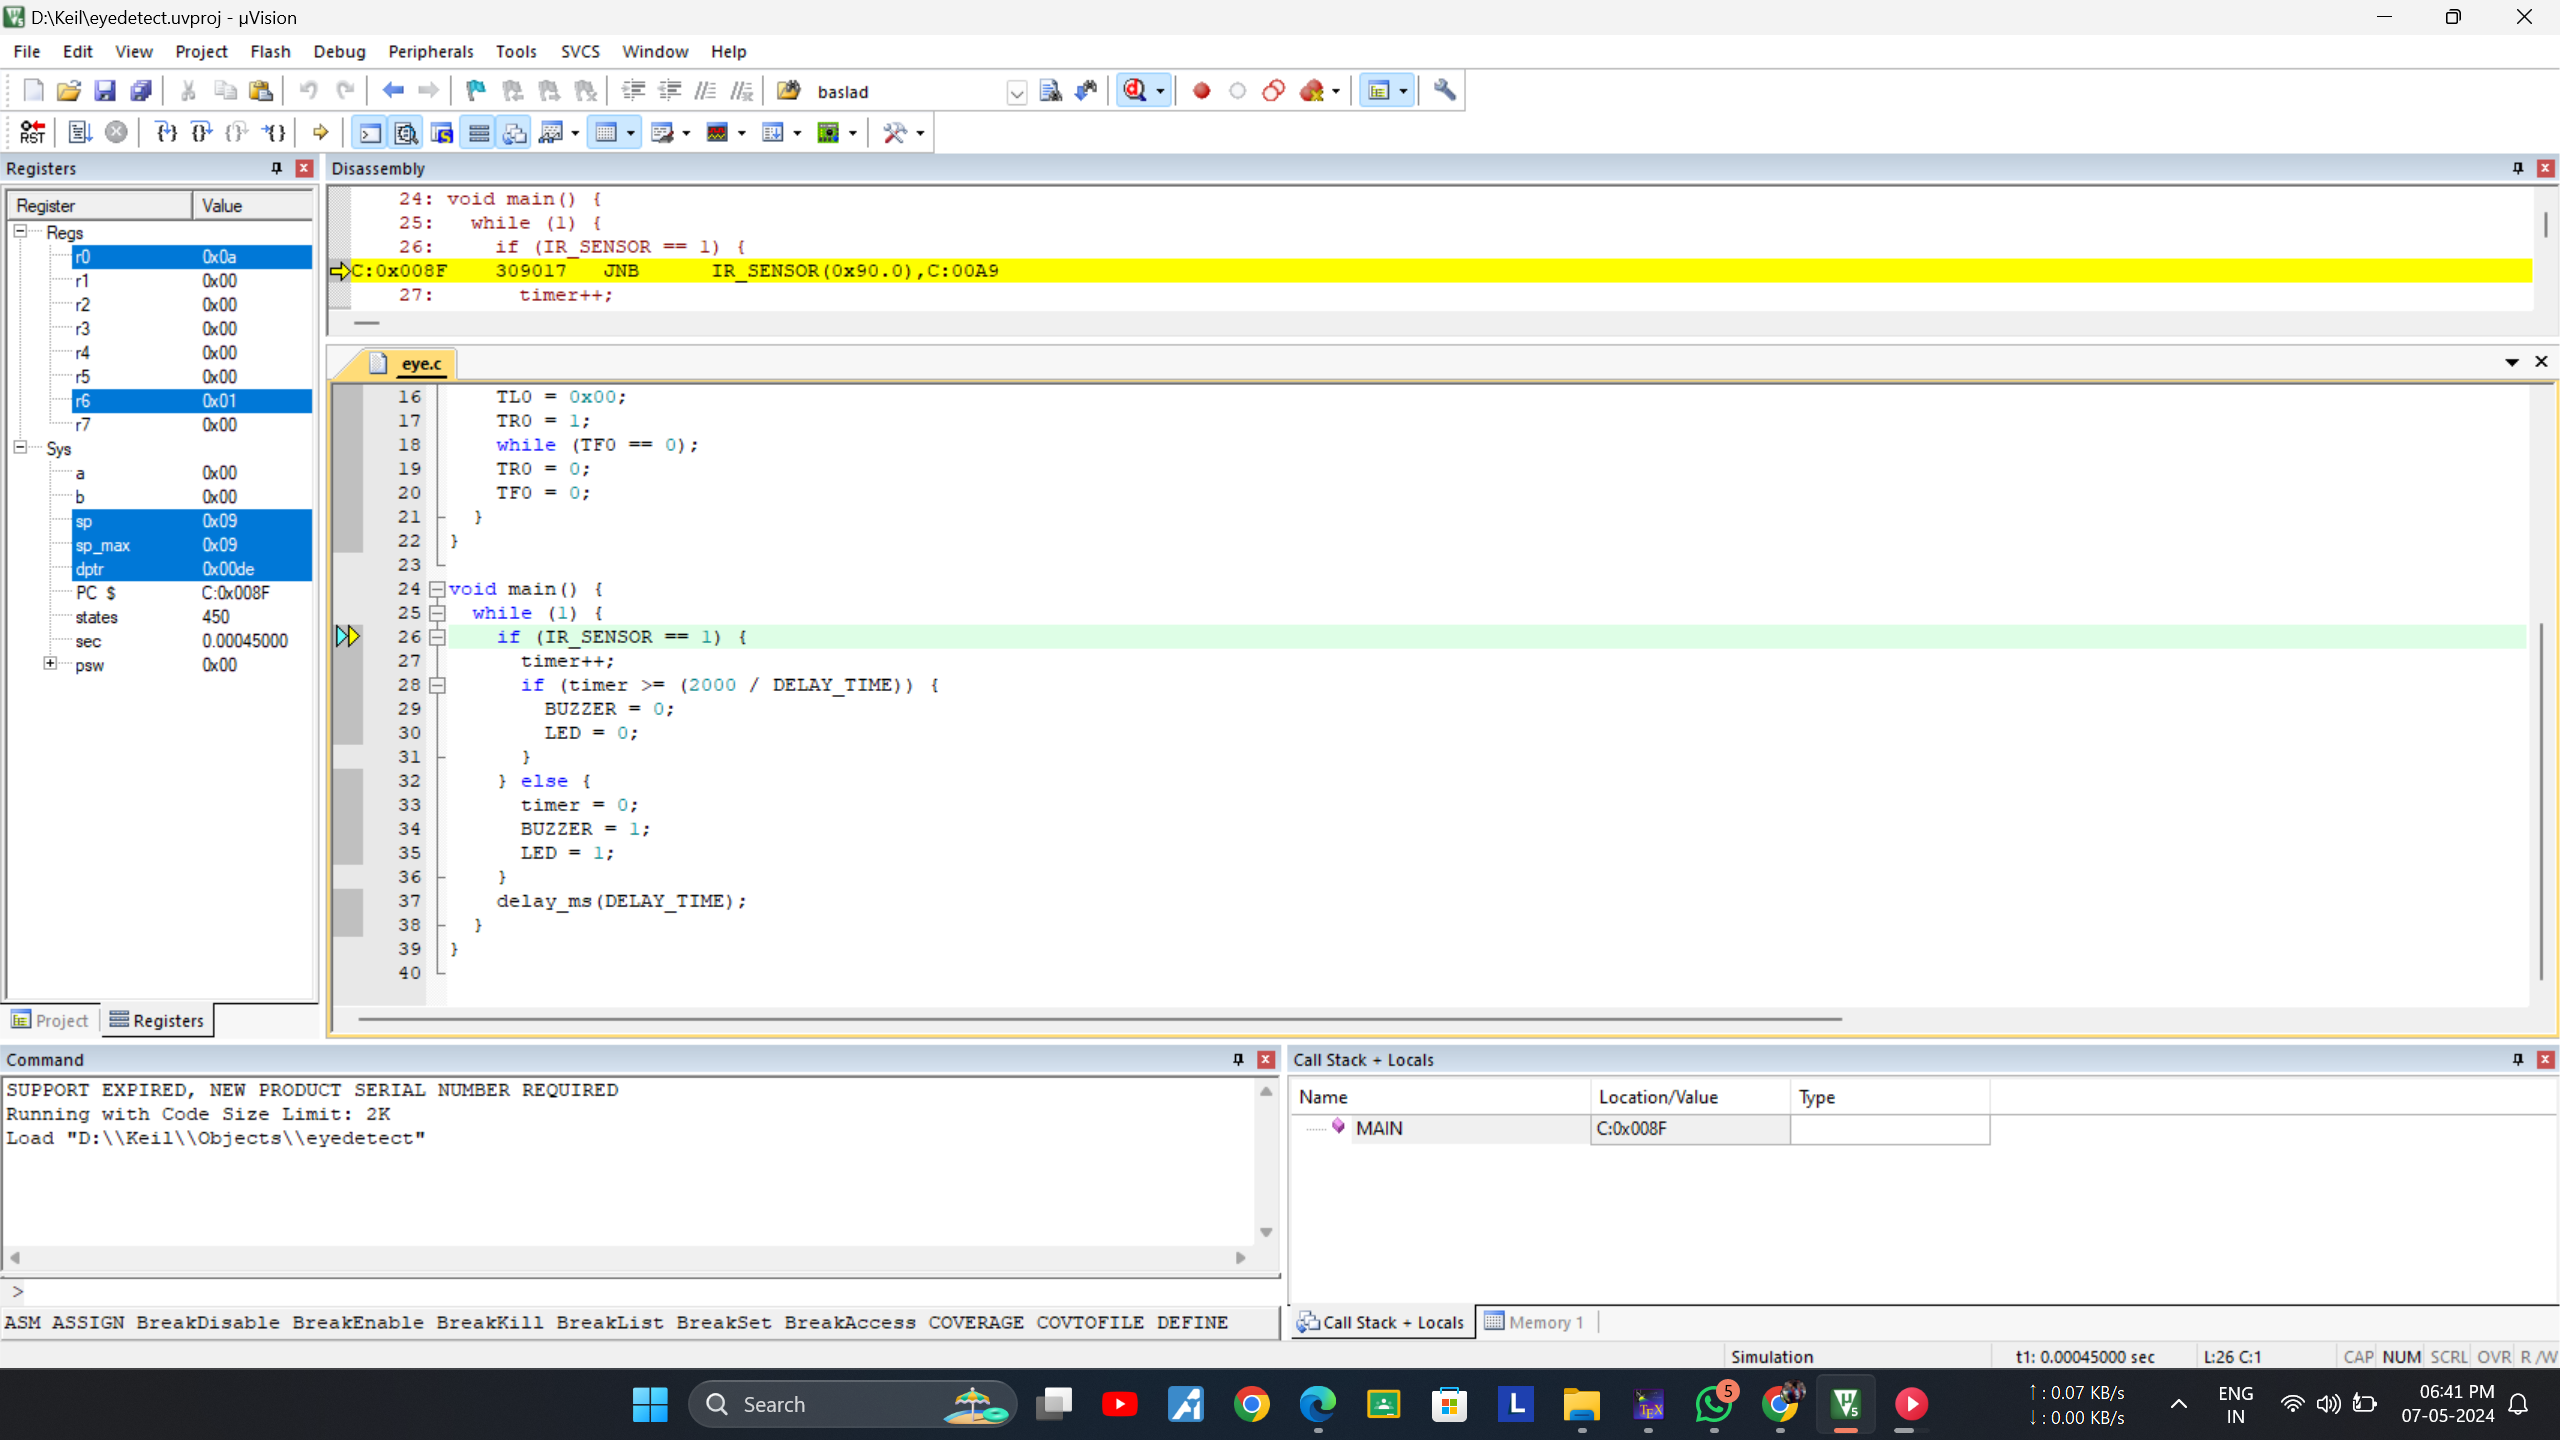
\includegraphics[width=\linewidth]{debugging}
		\caption{Code debugging}
		\label{fig:2}
	\end{subfigure}
	\caption{Code debugging and execution}
	\label{wave}
\end{figure}
\subsection{Generating hex file}
hex file is generated for buring code to AT89S51 microcontroller hex file is created
after every error is rectified
\begin{figure}[h!]
	\centering
	\begin{subfigure}[b]{0.4\textwidth}
		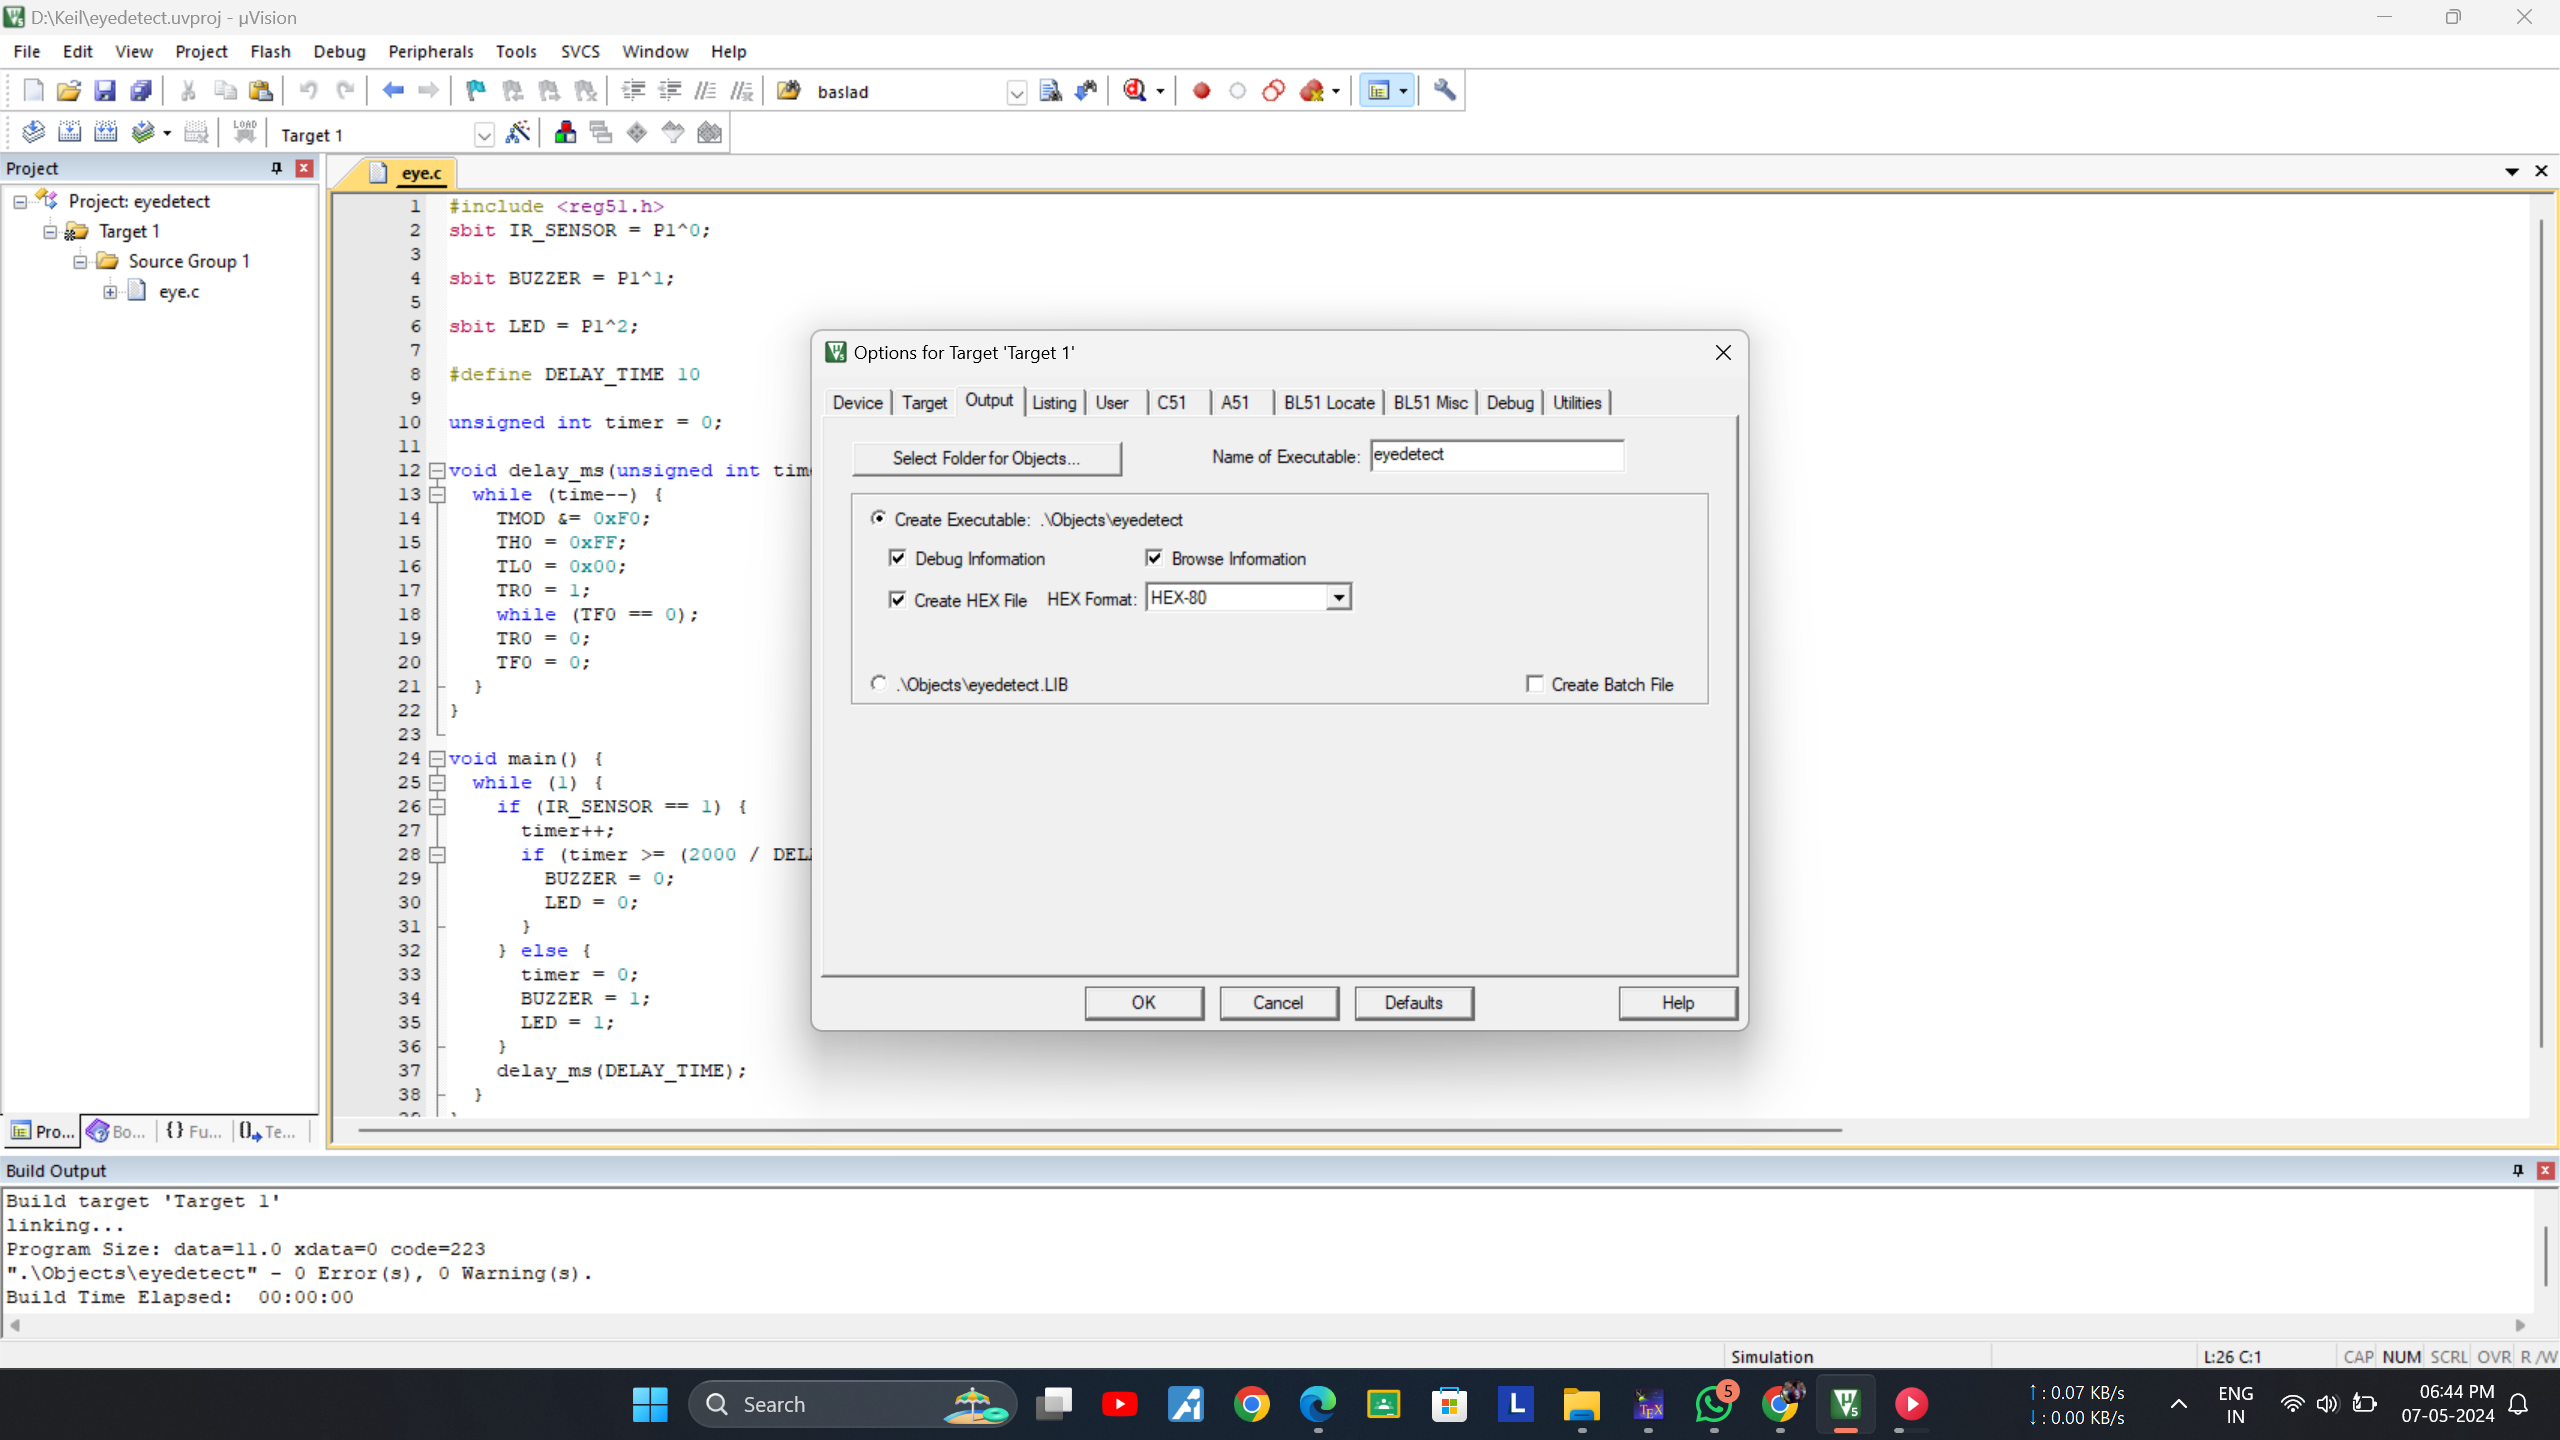
\includegraphics[width=\textwidth]{hex}
		\caption{creating hex file}
		\label{fig:1}
	\end{subfigure}
	\hspace{20mm}
	\begin{subfigure}[b]{0.4\textwidth}
		\includegraphics[width=\linewidth]{heXgen}
		\caption{hex file generated}
		\label{fig:2}
	\end{subfigure}
	\caption{HEX FILE GENERATION}
	\label{wave}
\end{figure}
\section{BURNING CODE TO AT89S51}

\subsection{Arduino as ISP}
Set up the Arduino as an ISP: Connect the Arduino board to the computer and upload
the ArduinoISP sketch to the Arduino.
\subsection{Connecting Arduino with  AT89S51}
Connect the AT89S51: Make the necessary connections between the Arduino and
AT89S51 microcontroller. This typically involves connecting the SPI pins (MISO,
MOSI, SCK) of the Arduino to the corresponding pins of the AT89S51 (P1.6, P1.5,
P1.7). Additionally, connect the Reset pin (RST) of the Arduino to the Reset pin
(P3.5) of the AT89S51.
connect crystal oscillator,33uf capacitors to 18 and 19 pin of at89s51
connect reset circuit to the 9th pin of at89s51
\subsection{Uploading code to AT89S51}
avrdude.exe file is downloaded and stored and path of location is noted.
\begin{figure}[h!]
	\centering
	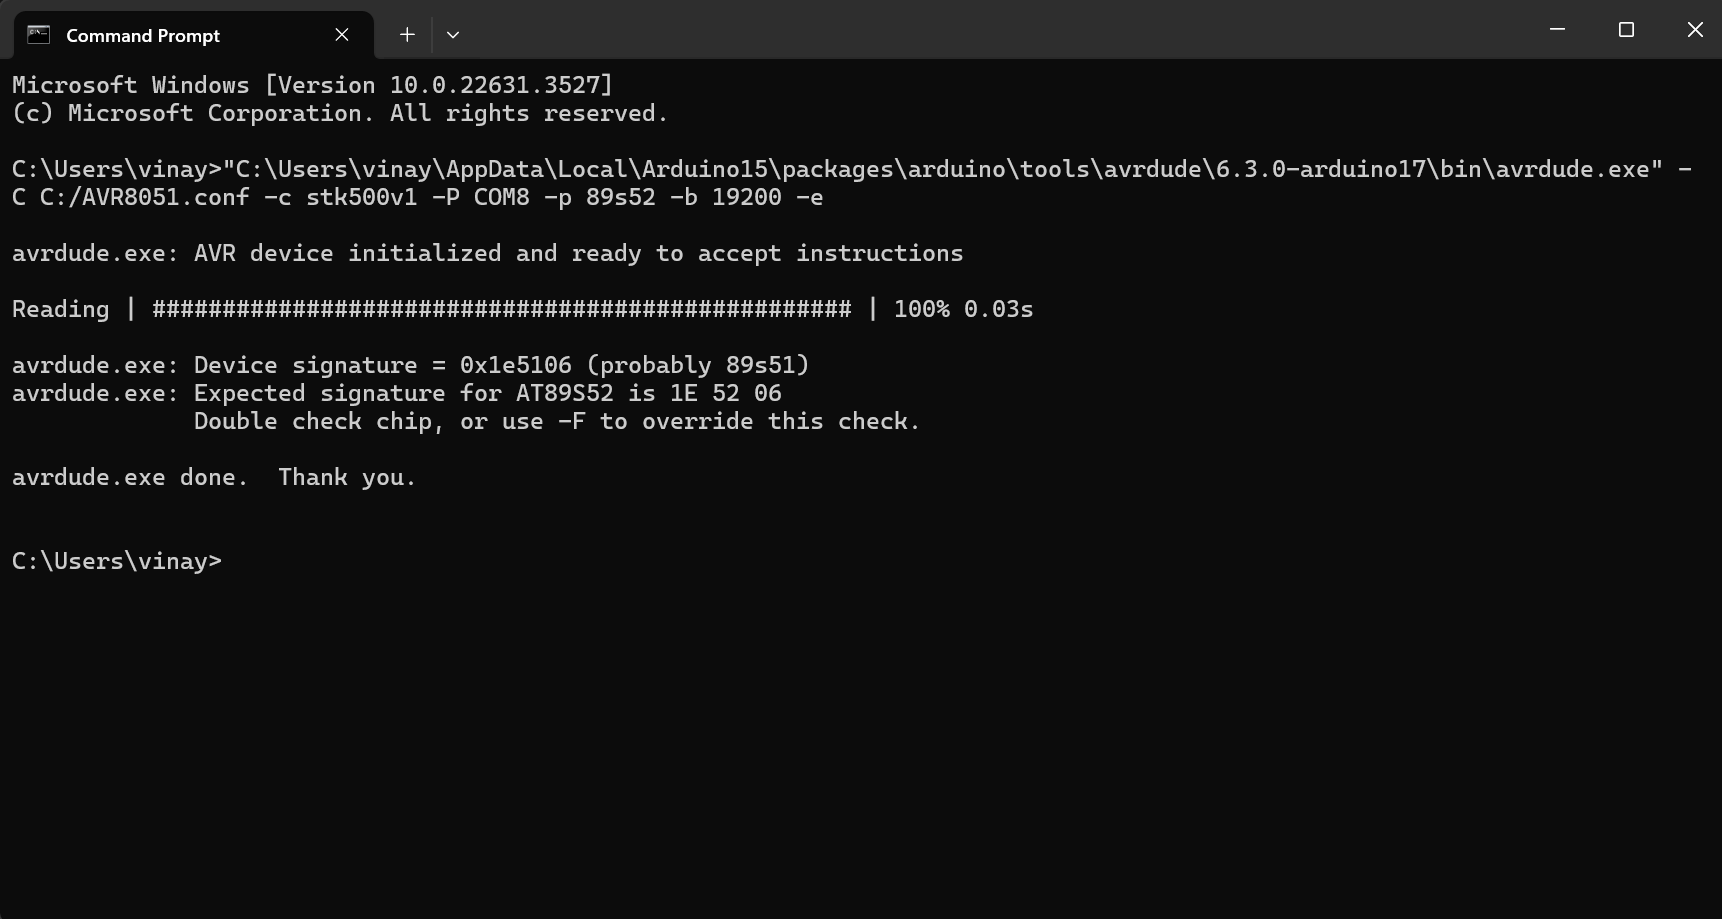
\includegraphics[width=.7\linewidth]{terminal}
	\caption{Burning of hexfile to AT89S51}
	\label{net2}
\end{figure}
\begin{figure}[h!]
	\centering
	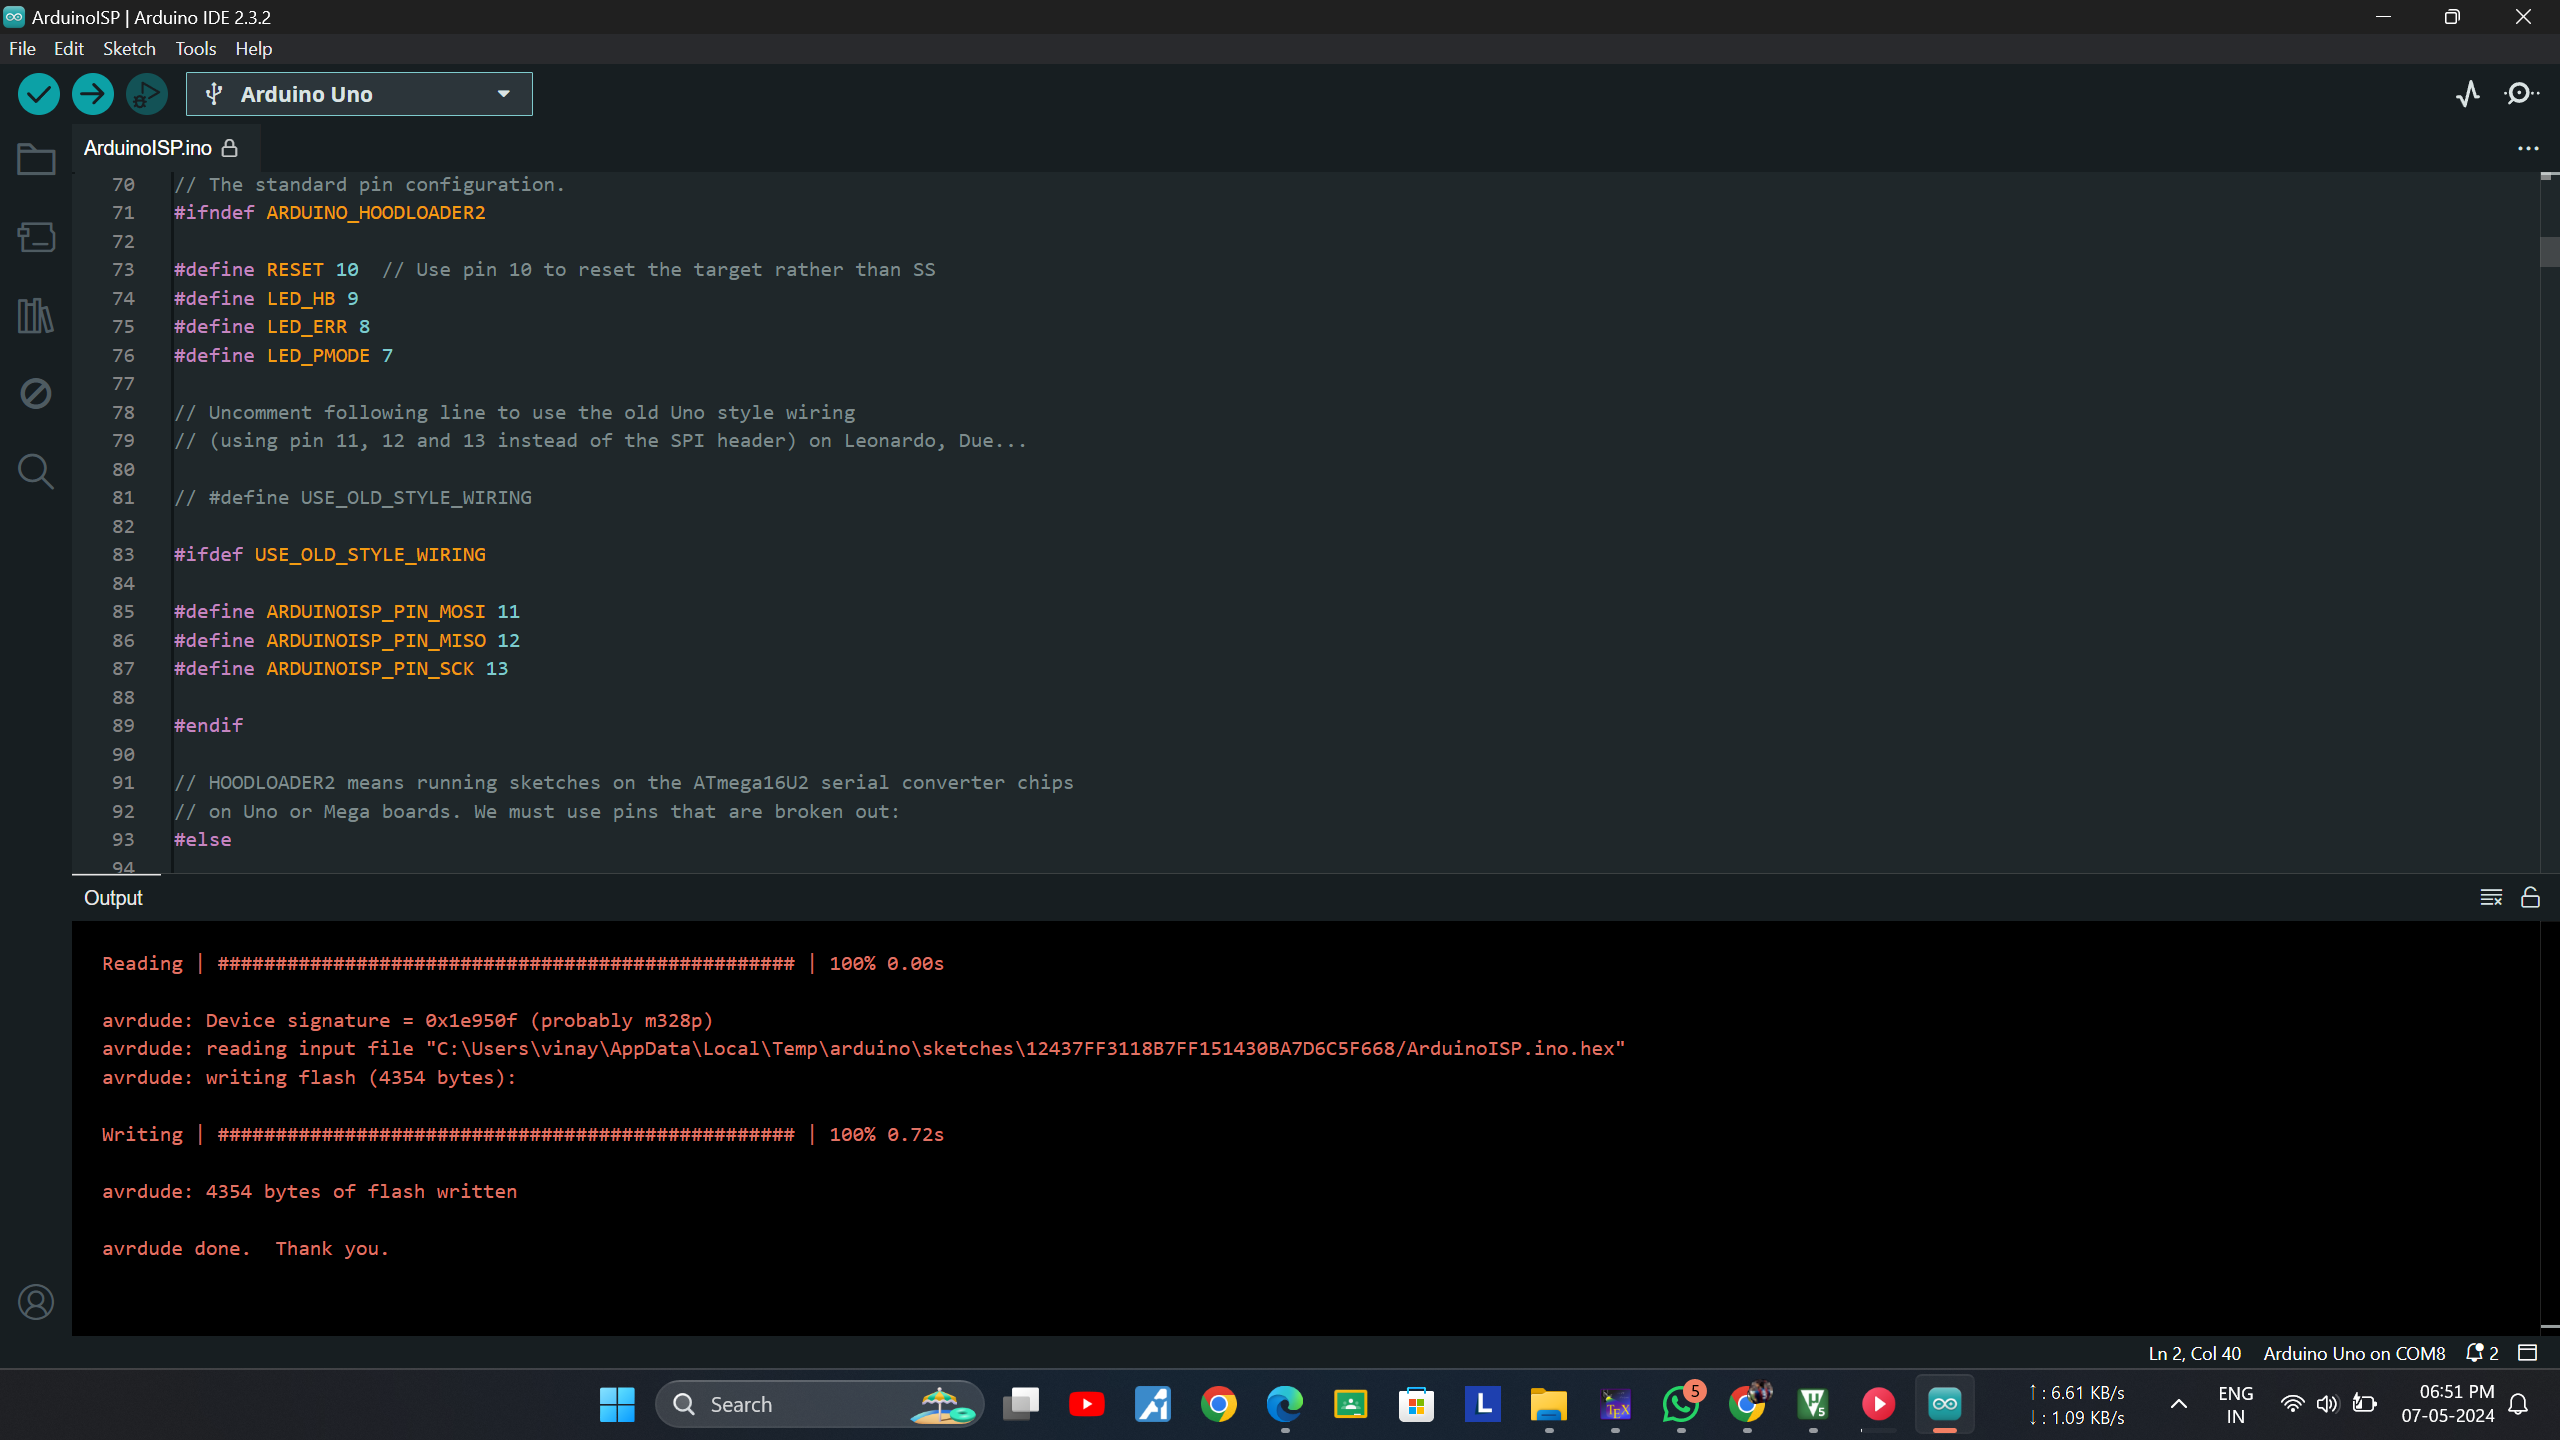
\includegraphics[width=.7\linewidth]{isp}
	\caption{Arduino as ISP}
	\label{net2}
\end{figure}
\begin{figure}[h!]
	\centering
	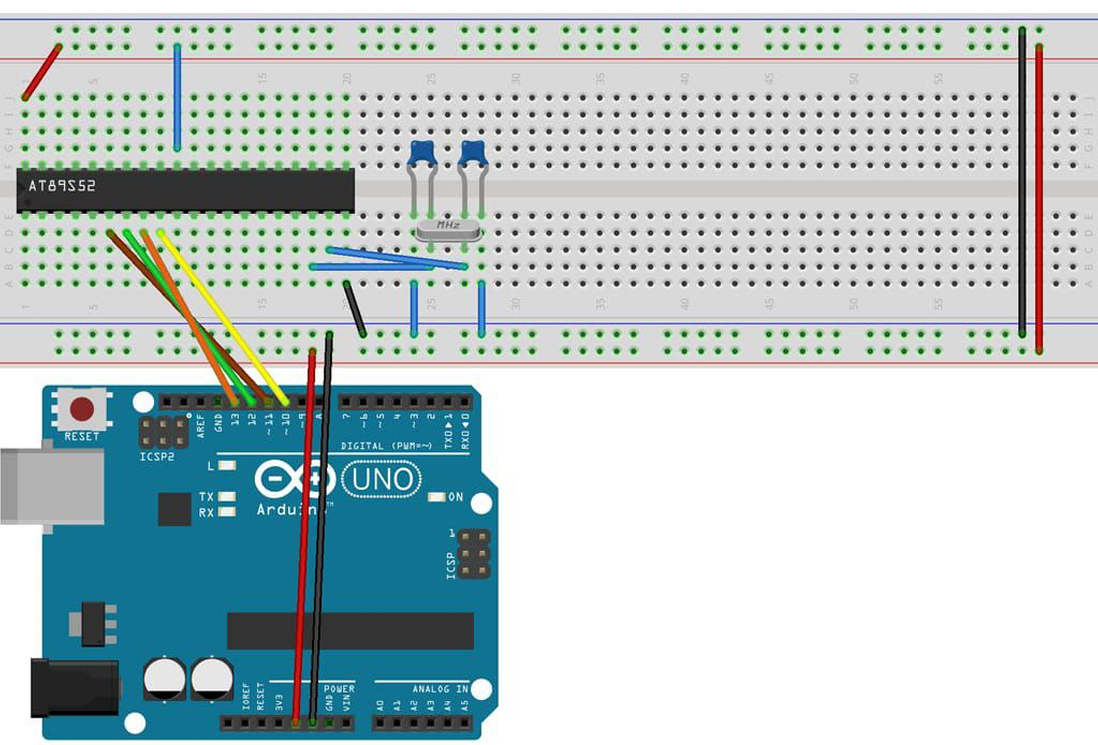
\includegraphics[width=.7\linewidth]{connection}
	\caption{Connection circuit}
	\label{net2}
\end{figure}
The location path of avrdude,microcontroller model(AT89S51 or AT89S52) ,output port number (arduino connected port) is inserted at corresponding places in the code in command
prompt window( as in figure below) and then the code is made to run and the hexfile is
burned to microcontroller
\section{PROJECT CIRCUIT AND TESTING}
For this project the components required are: 
\begin{enumerate}
	\item AT89S51 microcontroller
	\item IR sensor Module
	\item Breadboard
	\item Connecting wires
	\item Crystal Oscillator 11.0592 Mhz
	\item Capacitors (33pf,10uf)
	\item Resistor 10k	
	\item Buzzer
\end{enumerate}
\subsection{Circuit Connections}
\textbf{IR sensor:}The DOUT pin of the IR sensor module is connected to the 1st pin(PORT 1.0) of the Microcontroller. VCC, GND are connected to the 5V input and to the ground respectively.
\begin{figure}[h!]
	\centering
	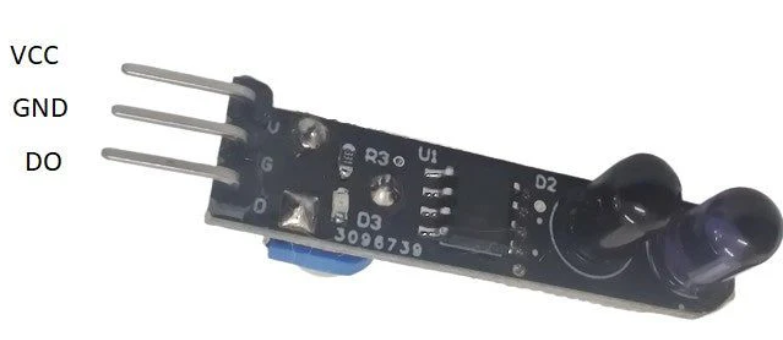
\includegraphics[width=.3\linewidth]{ir}
	\caption{IR Sensor Module}
	\label{net2}
\end{figure}\\
\textbf{Buzzer:}The anode of the buzzer is connected to 2nd pin (PORT 1.1) of the microcontroller. Cathode connected to the GND.
\begin{figure}[h!]
	\centering
	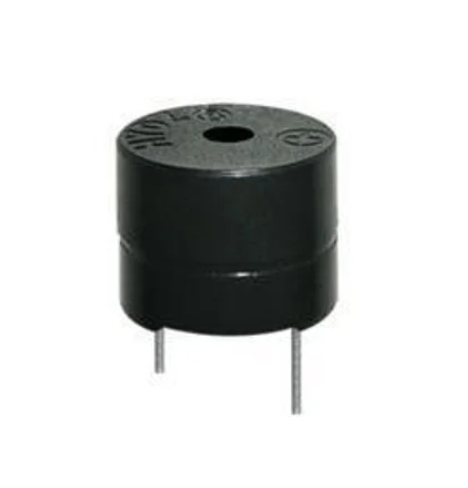
\includegraphics[width=.3\linewidth]{buzzer}
	\caption{Buzzer}
	\label{net2}
\end{figure}\\
\textbf{Other connections:}Vcc of the microcontroller shorted with 31th pin (EA pin).
Crystall Oscillator is connected to 18th,19th pin of MC.
\begin{figure}[h!]
	\centering
	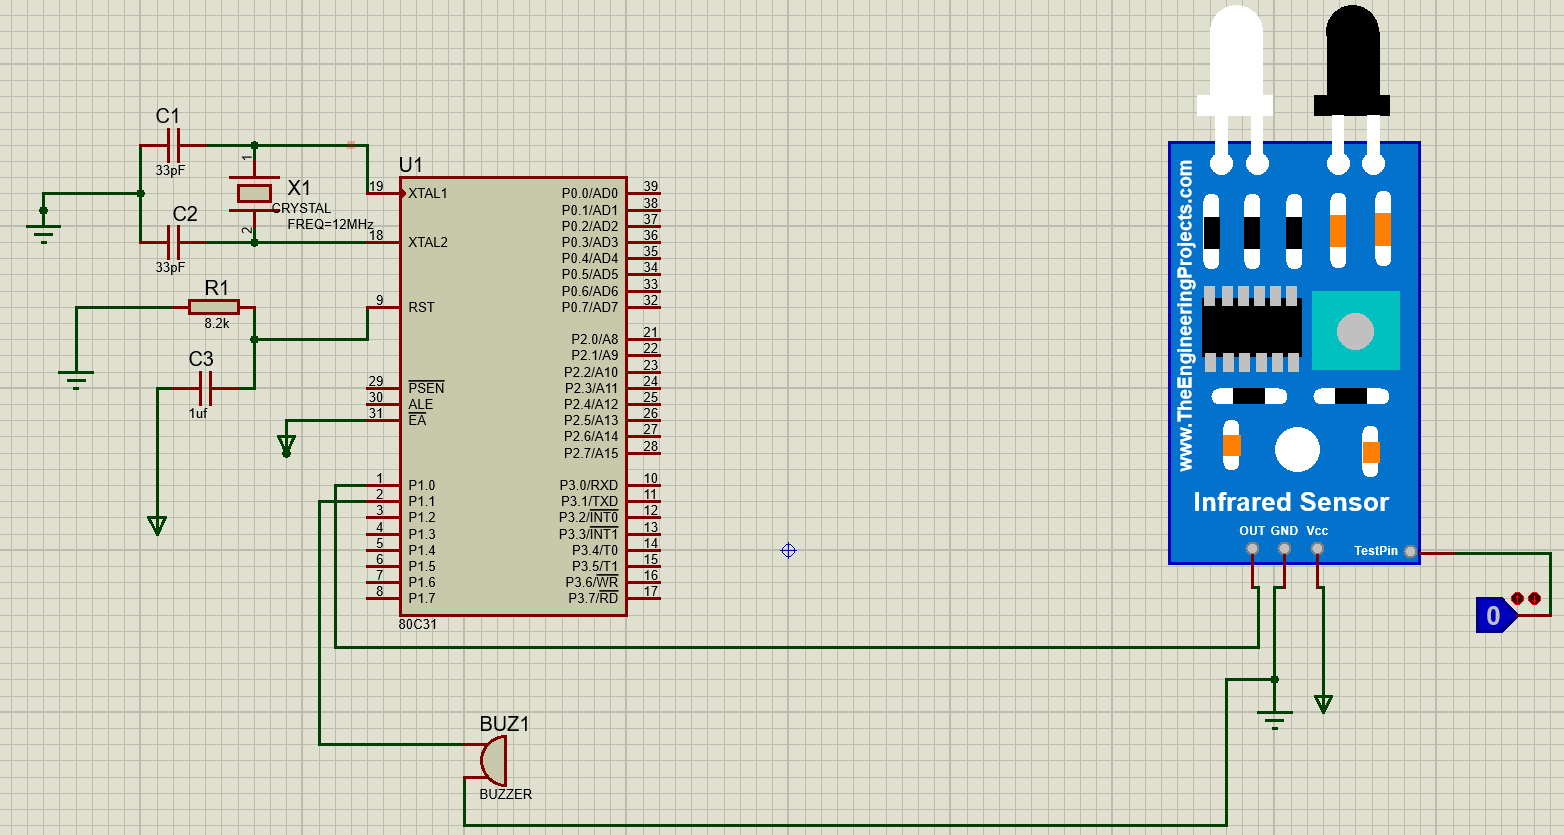
\includegraphics[width=1\linewidth]{proteus}
	\caption{Circuit Diagram}
	\label{net2}
\end{figure}
\begin{figure}[h!]
	\centering
	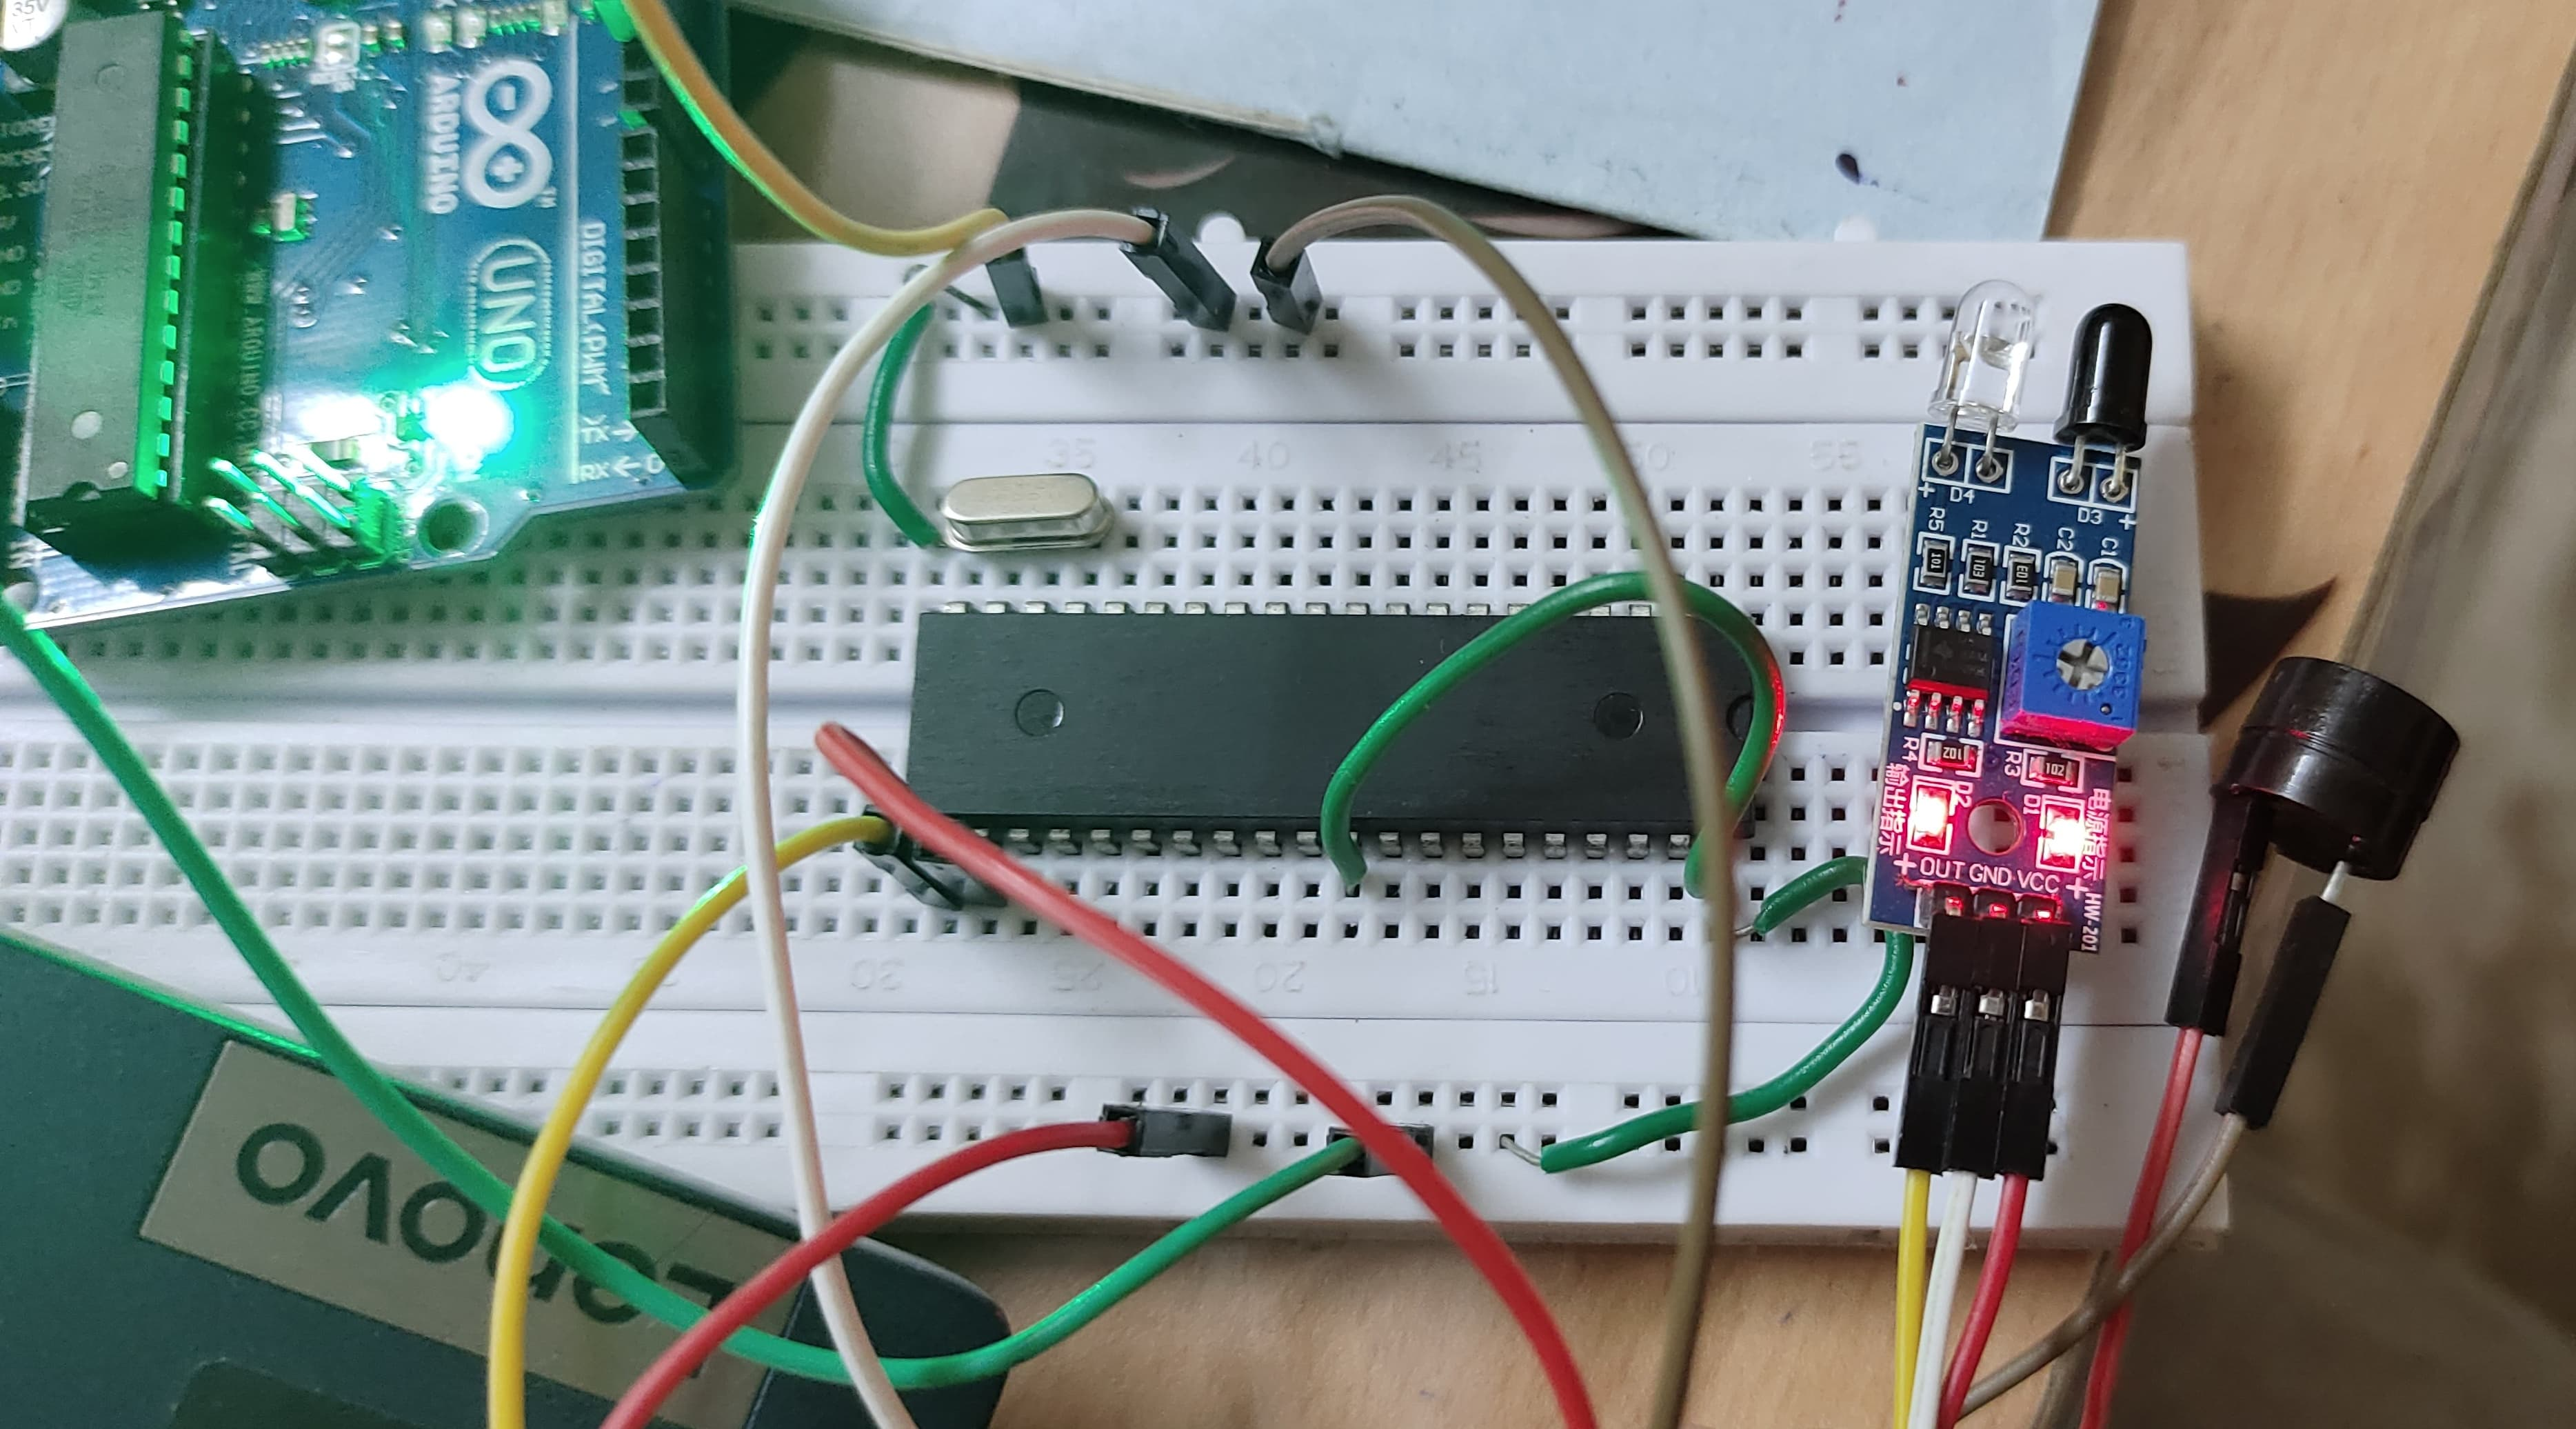
\includegraphics[width=1\linewidth]{circuit}
	\caption{Circuit}
	\label{net2}
\end{figure}\\
\subsection{Working of Code}
The IR sensor is connected to pin P1.0, and a buzzer is connected to pin P1.1.
The code defines a delay time constant and initializes a timer variable.
A delayms function generates delays in milliseconds using Timer 0.
In the main loop, the program continuously checks the IR sensor's status.
If an object is detected, the timer is incremented.
If the timer reaches a certain value (2 seconds), the buzzer is turned off.
If no object is detected, the timer is reset, and the buzzer is turned on.
Timer 0 is used to create the delay, operating in 16-bit mode.
The program waits for Timer 0 to overflow to indicate that the delay has elapsed.
Timer 0 is then stopped, and the overflow flag is cleared for the next operation.


%%********************Chapter 3**********
\chapter{Conclusion}
This project successfully developed a microcontroller-based drowsy driver detection system using an infrared (IR) sensor. The system leverages the principle that closed eyes alter the reflection of IR light, allowing the 8051 microcontroller to detect drowsiness based on sensor readings. When closed-eye detection persists for a predetermined period, the system triggers an audible alert via a buzzer. This immediate and clear notification aims to jolt the driver back to alertness and encourage them to take corrective action.

The project demonstrates the feasibility of a simple and cost-effective solution for mitigating drowsy driving risks. The system offers several advantages, including:\\
\textbf{Affordability:} The use of an IR sensor and 8051 microcontroller keeps the system cost-effective.
Ease of Use: The system requires minimal user interaction and no additional visual displays within the vehicle.\\
\textbf{Driver Focus:} The immediate and unavoidable buzzer alert directly addresses the driver's state of alertness.
\section{APPLICATIONS}
\begin{itemize}
	\item\textbf{Commercial Trucking Industry:} Enforced regulations and long haul journeys make truck drivers particularly susceptible to fatigue. This system can be integrated into commercial trucks to provide timely alerts and potentially link to fleet management systems for monitoring driver behavior.
	\item\textbf{Public Transportation:} Bus drivers and train operators navigate long routes and potentially monotonous schedules. Integrating this system into public transportation vehicles can enhance safety for both drivers and passengers.
	\item\textbf{Long-Distance Driving Scenarios:} Road trips or journeys on isolated highways can lead to driver drowsiness. This system can be a valuable addition to rental cars or personal vehicles used for long-distance travel.
	\item\textbf{Off-Road Applications:} Construction vehicles, agricultural equipment, and mining machinery often operate in demanding environments with long shifts. This system can be adapted for such vehicles to improve operator alertness and safety.
	\item\textbf{Driver Training and Monitoring Systems:} Driving schools and professional driver training programs can incorporate this system as a training tool to help drivers recognize and address drowsiness symptoms. Additionally, fleet management companies can utilize this technology for real-time monitoring and intervention when drowsiness is detected.
\end{itemize}

%%********************Chapter 4**********
\chapter{Bill of Materials}
\begin{table}[h]
	\centering
	\begin{tabular}{|l|l|l|l|l|l|}
		\hline
		SI.No & Item                   & Manufacturer        & Price/Unit (Rs.) & Quantity & Cost (Rs.) \\ \hline
		1     & 80S51                  & Atmel               & 150              & 1        & 150        \\ \hline
		2     & Capacitor(33pF)        & Keltron             & 1                & 2        & 2          \\ \hline
		3     & Capacitor(10uf)        & Keltron             & 10               & 1        & 10         \\ \hline
		4     & Breadboard             & Esel International  & 90               & 1        & 90         \\ \hline
		5     & Buzzer                 & Electronic Spices   & 15               & 1        & 15         \\ \hline
		6     & IR sensor              & Generic             & 150              & 1        & 150        \\ \hline
		7     & Oscillator(11.0592MHz) & Generic             & 8                & 1        & 8          \\ \hline
		8     & Resistor(10k)          & Elevctronic devices & 2                & 1        & 2          \\ \hline
	\end{tabular}
\end{table}

%%********************Chapter 5**********
\chapter{Code}


%% Include the C code
\lstinputlisting[language={C},caption=Source code of the project]{code/eye.c}


%%********************References**********
%%****This template uses IEEE bibliography style

 \begin{thebibliography}{99}
	\bibitem{india} Gemini AI, ChatGPT
	
	
	\bibitem{rpi} https://www.electronicsforu.com/technology-trends/learn-electronics/ir-led-infrared-sensor-basics
	
	\bibitem{japan} https://www.tutorialspoint.com/microprocessor/microcontrollers-8051-pin-description.html		
\end{thebibliography}

\end{document}